\documentclass[10pt,a4paper,twocolumn]{article}

% ── Encoding & Language ──────────────────────────────────────────────────────
\usepackage[utf8]{inputenc}
\usepackage[T1]{fontenc}

% ── Layout ───────────────────────────────────────────────────────────────────
\usepackage[top=2.3cm, bottom=2.3cm, left=2.0cm, right=2.0cm]{geometry}
\usepackage{setspace}
\setstretch{1.08}
\usepackage{indentfirst}
\setlength{\parindent}{1.25cm}
\setlength{\parskip}{0pt}
\setlength{\columnsep}{0.7cm}
\setlength{\emergencystretch}{3em}

% ── Fonts & Typography ───────────────────────────────────────────────────────
\usepackage{lmodern}
\usepackage{microtype}

% ── Graphics & Tables ────────────────────────────────────────────────────────
\usepackage{graphicx}
\usepackage{booktabs}
\usepackage{caption}
\usepackage{subcaption}
\usepackage{float}
\usepackage{array}
\usepackage{xcolor}
\usepackage{tabularx}

% ── Math ─────────────────────────────────────────────────────────────────────
\usepackage{amsmath}

% ── Hyperlinks ───────────────────────────────────────────────────────────────
\usepackage[hidelinks,hypertexnames=false]{hyperref}
\renewcommand{\contentsname}{Sumário}

% ── Headers & Footers ────────────────────────────────────────────────────────
\usepackage{fancyhdr}
\pagestyle{fancy}
\fancyhf{}
\fancyhead[L]{\small Laboratório de Experimentação de Software}
\fancyhead[R]{\small PUC Minas -- 2026/1}
\fancyfoot[C]{\thepage}
\setlength{\headheight}{14pt}
\renewcommand{\headrulewidth}{0.4pt}

% ─────────────────────────────────────────────────────────────────────────────
\begin{document}

\onecolumn

% ── Capa ─────────────────────────────────────────────────────────────────────
\begin{titlepage}
  \centering
  \vspace*{2.0cm}

  {\normalsize
    Pontifícia Universidade Católica de Minas Gerais (PUC~Minas)\\
    Laboratório de Experimentação de Software -- 2026/1
  }

  \vspace*{2.8cm}

  {\large
    Raphael Brito\\[0.3em]
    Yan Cota
  }

  \vspace*{4.2cm}

  {\LARGE \textbf{Laboratório 05}\\[0.5em]
  \Large GraphQL vs.\ REST: Um Experimento Controlado}

  \vspace*{0.6em}
  {\normalsize Estudo de tempo de resposta e tamanho de payload na API do GitHub}

  \vfill

  {\normalsize Belo Horizonte\\ 2026}
\end{titlepage}

% ── Sumário ──────────────────────────────────────────────────────────────────
\pagenumbering{roman}
\tableofcontents
\newpage
\pagenumbering{arabic}
\setcounter{page}{1}
\twocolumn

% ─────────────────────────────────────────────────────────────────────────────
\section{Introdução}
% ─────────────────────────────────────────────────────────────────────────────

A escolha do estilo arquitetural de uma API influencia diretamente o
desempenho percebido e o consumo de recursos de uma aplicação. O modelo
\textbf{REST}, predominante há mais de uma década, expõe recursos em
\textit{endpoints} fixos que retornam representações completas, frequentemente
incorrendo em \textit{over-fetching} -- o transporte de campos que o cliente
não utilizará. O \textbf{GraphQL}, por sua vez, permite ao cliente declarar
exatamente quais campos deseja, prometendo respostas mais enxutas.

Neste laboratório conduzimos um \textbf{experimento controlado} comparando os
dois paradigmas na API pública do GitHub, tendo como objeto experimental o
repositório do motor de xadrez de código aberto
\texttt{official-stockfish/Stockfish}. Duas variáveis de resposta foram
medidas em cada requisição: a \textbf{latência} (tempo de ida e volta, em
milissegundos) e o \textbf{tamanho do payload} (em bytes). Ao todo foram
consolidadas \textbf{487 medições válidas} (HTTP 200), distribuídas entre os
quatro tipos de recurso avaliados.

A motivação central é verificar empiricamente se a vantagem conceitual do
GraphQL -- evitar o \textit{over-fetching} -- se traduz em ganhos
estatisticamente significativos de \emph{banda} e de \emph{tempo}, e em que
medida tais ganhos dependem do recurso consultado.

% ─────────────────────────────────────────────────────────────────────────────
\section{Questões de Pesquisa e Hipóteses}
% ─────────────────────────────────────────────────────────────────────────────

O experimento responde a duas questões de pesquisa:

\begin{description}
  \item[\textbf{RQ1 -- Tempo de resposta}] As respostas às consultas GraphQL
    são mais rápidas (menor latência) do que às consultas REST?
  \item[\textbf{RQ2 -- Tamanho do payload}] As respostas às consultas GraphQL
    possuem tamanho menor (em bytes) do que às consultas REST?
\end{description}

Para cada questão formulamos hipóteses nula ($H_0$) e alternativa ($H_1$),
testadas de forma \textbf{unilateral} (esperamos que o GraphQL seja
\emph{menor} em ambas as métricas):

\paragraph{RQ1 (latência).}
\begin{align*}
  H_{0,1}&: \text{Latência}_{\text{GraphQL}} \geq \text{Latência}_{\text{REST}}\\
  H_{1,1}&: \text{Latência}_{\text{GraphQL}} < \text{Latência}_{\text{REST}}
\end{align*}

\paragraph{RQ2 (tamanho).}
\begin{align*}
  H_{0,2}&: \text{Tamanho}_{\text{GraphQL}} \geq \text{Tamanho}_{\text{REST}}\\
  H_{1,2}&: \text{Tamanho}_{\text{GraphQL}} < \text{Tamanho}_{\text{REST}}
\end{align*}

Nossa expectativa inicial é que $H_{1,2}$ seja fortemente confirmada (o
GraphQL transfere apenas os campos solicitados), enquanto $H_{1,1}$ seja
apenas \emph{parcialmente} confirmada, pois a latência depende também de
fatores de rede e de processamento do servidor que não favorecem
intrinsecamente nenhum dos paradigmas.

% ─────────────────────────────────────────────────────────────────────────────
\section{Objetivos}
% ─────────────────────────────────────────────────────────────────────────────

\subsection{Objetivo Geral}

Avaliar quantitativamente, sob rigor estatístico, os impactos de desempenho
(latência) e de eficiência de rede (tamanho de payload) decorrentes da escolha
entre GraphQL e REST na API do GitHub.

\subsection{Objetivos Específicos}

\begin{itemize}
  \item Comparar as distribuições de latência e de tamanho entre os dois
    paradigmas, por recurso, com o teste de Mann-Whitney~U unilateral.
  \item Quantificar a magnitude prática das diferenças por meio do tamanho de
    efeito \textit{Cliff's Delta}.
  \item Mensurar a economia de banda absoluta (bytes trafegados) ao longo de
    todo o experimento.
  \item Documentar o procedimento de forma a permitir reprodução e replicação
    integrais.
\end{itemize}

% ─────────────────────────────────────────────────────────────────────────────
\section{Metodologia}
% ─────────────────────────────────────────────────────────────────────────────

\subsection{Desenho do Experimento}

Adotou-se um projeto \textbf{dentro de sujeitos} (\textit{within-subject}),
em que o mesmo objeto experimental é submetido aos dois tratamentos. As
\textbf{variáveis independentes} são: (i)~o \emph{paradigma de API}
(REST ou GraphQL) e (ii)~o \emph{tipo de recurso} consultado, com quatro
níveis -- \texttt{repo} (metadados do repositório), \texttt{commits},
\texttt{issues} e \texttt{pulls} (listas dos 30 itens mais recentes). As
\textbf{variáveis dependentes} são a latência ($Y_1$, em ms) e o tamanho do
payload ($Y_2$, em bytes).

\paragraph{Tratamentos.} O tratamento REST consiste em requisições
\texttt{HTTP GET} aos \textit{endpoints} da API REST v3. O tratamento GraphQL
consiste em requisições \texttt{HTTP POST} à API GraphQL v4, cujas
\textit{queries} solicitam estritamente o mesmo conjunto lógico de campos que
seria exibido em uma interface, evitando o \textit{over-fetching}.

\paragraph{Randomização e intercalação.} Para isolar fatores de confusão
(oscilações de rede, flutuações temporais do servidor e \textit{cache} de
rota), todas as requisições de uma execução são embaralhadas
(\texttt{random.shuffle}) e \textbf{intercaladas}, de modo que REST e GraphQL
nunca sejam medidos em rajadas separadas.

\paragraph{Tamanho amostral.} O desenho prevê $N \geq 30$ medições por
combinação (tratamento $\times$ recurso), satisfazendo o Teorema do Limite
Central. Nesta execução consolidada obtivemos \textbf{487 medições válidas}
(todas com status HTTP 200), entre 60 e 62 por célula, sendo 243 requisições
REST e 244 GraphQL.

\subsection{Ambiente de Execução dos Trials}

Para permitir reprodução, registramos o ambiente em que os \textit{trials}
foram realizados:

\begin{itemize}
  \item \textbf{Linguagem/runtime:} Python 3.8+.
  \item \textbf{Bibliotecas:} \texttt{requests} (cliente HTTP),
    \texttt{scipy} (testes estatísticos), \texttt{pandas} (processamento),
    \texttt{matplotlib}/\texttt{seaborn} (gráficos) e
    \texttt{python-dotenv} (configuração).
  \item \textbf{Medição de latência:} \texttt{time.perf\_counter()}
    envolvendo a chamada, medindo o RTT completo do lado do cliente.
  \item \textbf{Medição de tamanho:} \texttt{len(response.content)}, isto é,
    o número de bytes do corpo da resposta.
  \item \textbf{Autenticação:} \textit{Personal Access Token} do GitHub
    (cabeçalho \texttt{Authorization: Bearer}), com
    \texttt{Cache-Control: no-cache} e \textit{User-Agent} dedicado.
  \item \textbf{Servidores:} infraestrutura de produção do GitHub
    (\texttt{api.github.com}), acessada por uma máquina cliente sob conexão de
    internet pública (banda larga).
  \item \textbf{Atraso entre chamadas:} 1{,}5\,s, evitando \textit{rate
    limiting} e rajadas consecutivas.
  \item \textbf{Janela de coleta:} 26 de junho de 2026
    (\textit{timestamps} registrados em UTC).
\end{itemize}

\subsection{Procedimento de Coleta e Análise}

O \textit{pipeline} é composto por quatro etapas, cada uma em um \textit{script}
dedicado no diretório \texttt{code/}:

\begin{enumerate}
  \item \texttt{collector.py} -- executa as requisições intercaladas e grava
    cada medição bem-sucedida em \texttt{data/raw\_data.csv}.
  \item \texttt{processor.py} -- consolida estatísticas descritivas por célula.
  \item \texttt{analyzer.py} -- aplica os testes de hipótese e gera o
    relatório estatístico.
  \item \texttt{visualizer.py} -- gera os gráficos comparativos.
\end{enumerate}

A análise estatística é \textbf{não-paramétrica}, justificada pelo teste de
normalidade de \textbf{Shapiro-Wilk}, que rejeitou a normalidade
($p < 0{,}001$) em todas as distribuições. Assim, empregamos:

\begin{itemize}
  \item \textbf{Teste U de Mann-Whitney} (unilateral, $H_1$: GraphQL
    $<$ REST), robusto a \textit{outliers}, ao nível de significância
    $\alpha = 0{,}05$.
  \item \textbf{Cliff's Delta} ($\delta$) como tamanho de efeito, interpretado
    como desprezível ($|\delta|<0{,}147$), pequeno ($<0{,}33$), médio
    ($<0{,}474$) ou grande ($\geq 0{,}474$).
\end{itemize}

A notação de significância adotada nas tabelas é: $p<0{,}001$ (***),
$p<0{,}01$ (**), $p<0{,}05$ (*) e $p\geq 0{,}05$ (ns).

\subsection{Reprodução e Replicação}

O experimento é integralmente reproduzível com os comandos:
\texttt{pip install -r requirements.txt}; cópia de \texttt{.env.example} para
\texttt{.env} com um \texttt{GITHUB\_TOKEN} válido; e execução sequencial de
\texttt{collector.py}, \texttt{processor.py}, \texttt{analyzer.py} e
\texttt{visualizer.py}. Os dados brutos, o relatório estatístico e os gráficos
ficam versionados em \texttt{code/data/} e \texttt{code/plots/}.

% ─────────────────────────────────────────────────────────────────────────────
\section{Resultados}
% ─────────────────────────────────────────────────────────────────────────────

A Tabela~\ref{tab:global} apresenta as medianas globais (todos os recursos
agregados) de cada métrica, por paradigma.

\begin{table}[H]
  \centering
  \caption{Medianas globais por paradigma (todos os recursos).}
  \label{tab:global}
  \small
  \begin{tabular}{lrr}
    \toprule
    \textbf{Métrica} & \textbf{GraphQL} & \textbf{REST} \\
    \midrule
    Latência (ms) & 534,79 & 615,32 \\
    Tamanho (bytes) & --- & --- \\
    \quad Tráfego total & 1,67\,MB & 35,04\,MB \\
    \bottomrule
  \end{tabular}
\end{table}

No total, o GraphQL trafegou \textbf{1,67\,MB} contra \textbf{35,04\,MB} do
REST -- uma \textbf{economia de banda de 95,2\%} ao longo do experimento.

% ─────────────────────────────────────────────────────────────────────────────
\subsection{RQ1 -- Tempo de resposta}
% ─────────────────────────────────────────────────────────────────────────────

A Tabela~\ref{tab:rq1} resume o teste de Mann-Whitney~U para a latência. O
resultado é \textbf{misto}: o GraphQL é significativamente mais rápido em
\texttt{issues} e \texttt{pulls}, mas \emph{não} há evidência de ganho em
\texttt{repo} e \texttt{commits}.

\begin{table}[H]
  \centering
  \caption{RQ1 -- Mann-Whitney U (unilateral, GraphQL $<$ REST) para latência.}
  \label{tab:rq1}
  \small
  \begin{tabular}{lrrrl}
    \toprule
    \textbf{Recurso} & \textbf{M.\ GQL} & \textbf{M.\ REST} & $\boldsymbol{\delta}$ & \textbf{Sig.} \\
    \midrule
    repo    & 503,2 & 595,0 & $-0,062$ & ns \\
    commits & 635,0 & 621,1 & $-0,125$ & ns \\
    issues  & 626,9 & 746,9 & $-0,262$ & ** \\
    pulls   & 581,7 & 853,6 & $-0,407$ & *** \\
    \bottomrule
  \end{tabular}
  \\[2pt]
  {\scriptsize M.\ = mediana (ms); $\delta$ = Cliff's Delta.
  ns: $p\geq0,05$; **: $p<0,01$; ***: $p<0,001$.}
\end{table}

A Figura~\ref{fig:latency} mostra os \textit{boxplots} de latência por recurso.
As distribuições são fortemente assimétricas e com \textit{outliers}, o que
reforça a escolha por testes não-paramétricos. Onde o payload REST é muito
volumoso (\texttt{pulls}, \texttt{issues}), o tempo de transferência também
cresce, e o GraphQL leva vantagem; em recursos pequenos (\texttt{repo}) ou de
custo de processamento semelhante (\texttt{commits}), a diferença desaparece.

\begin{figure}[H]
  \centering
  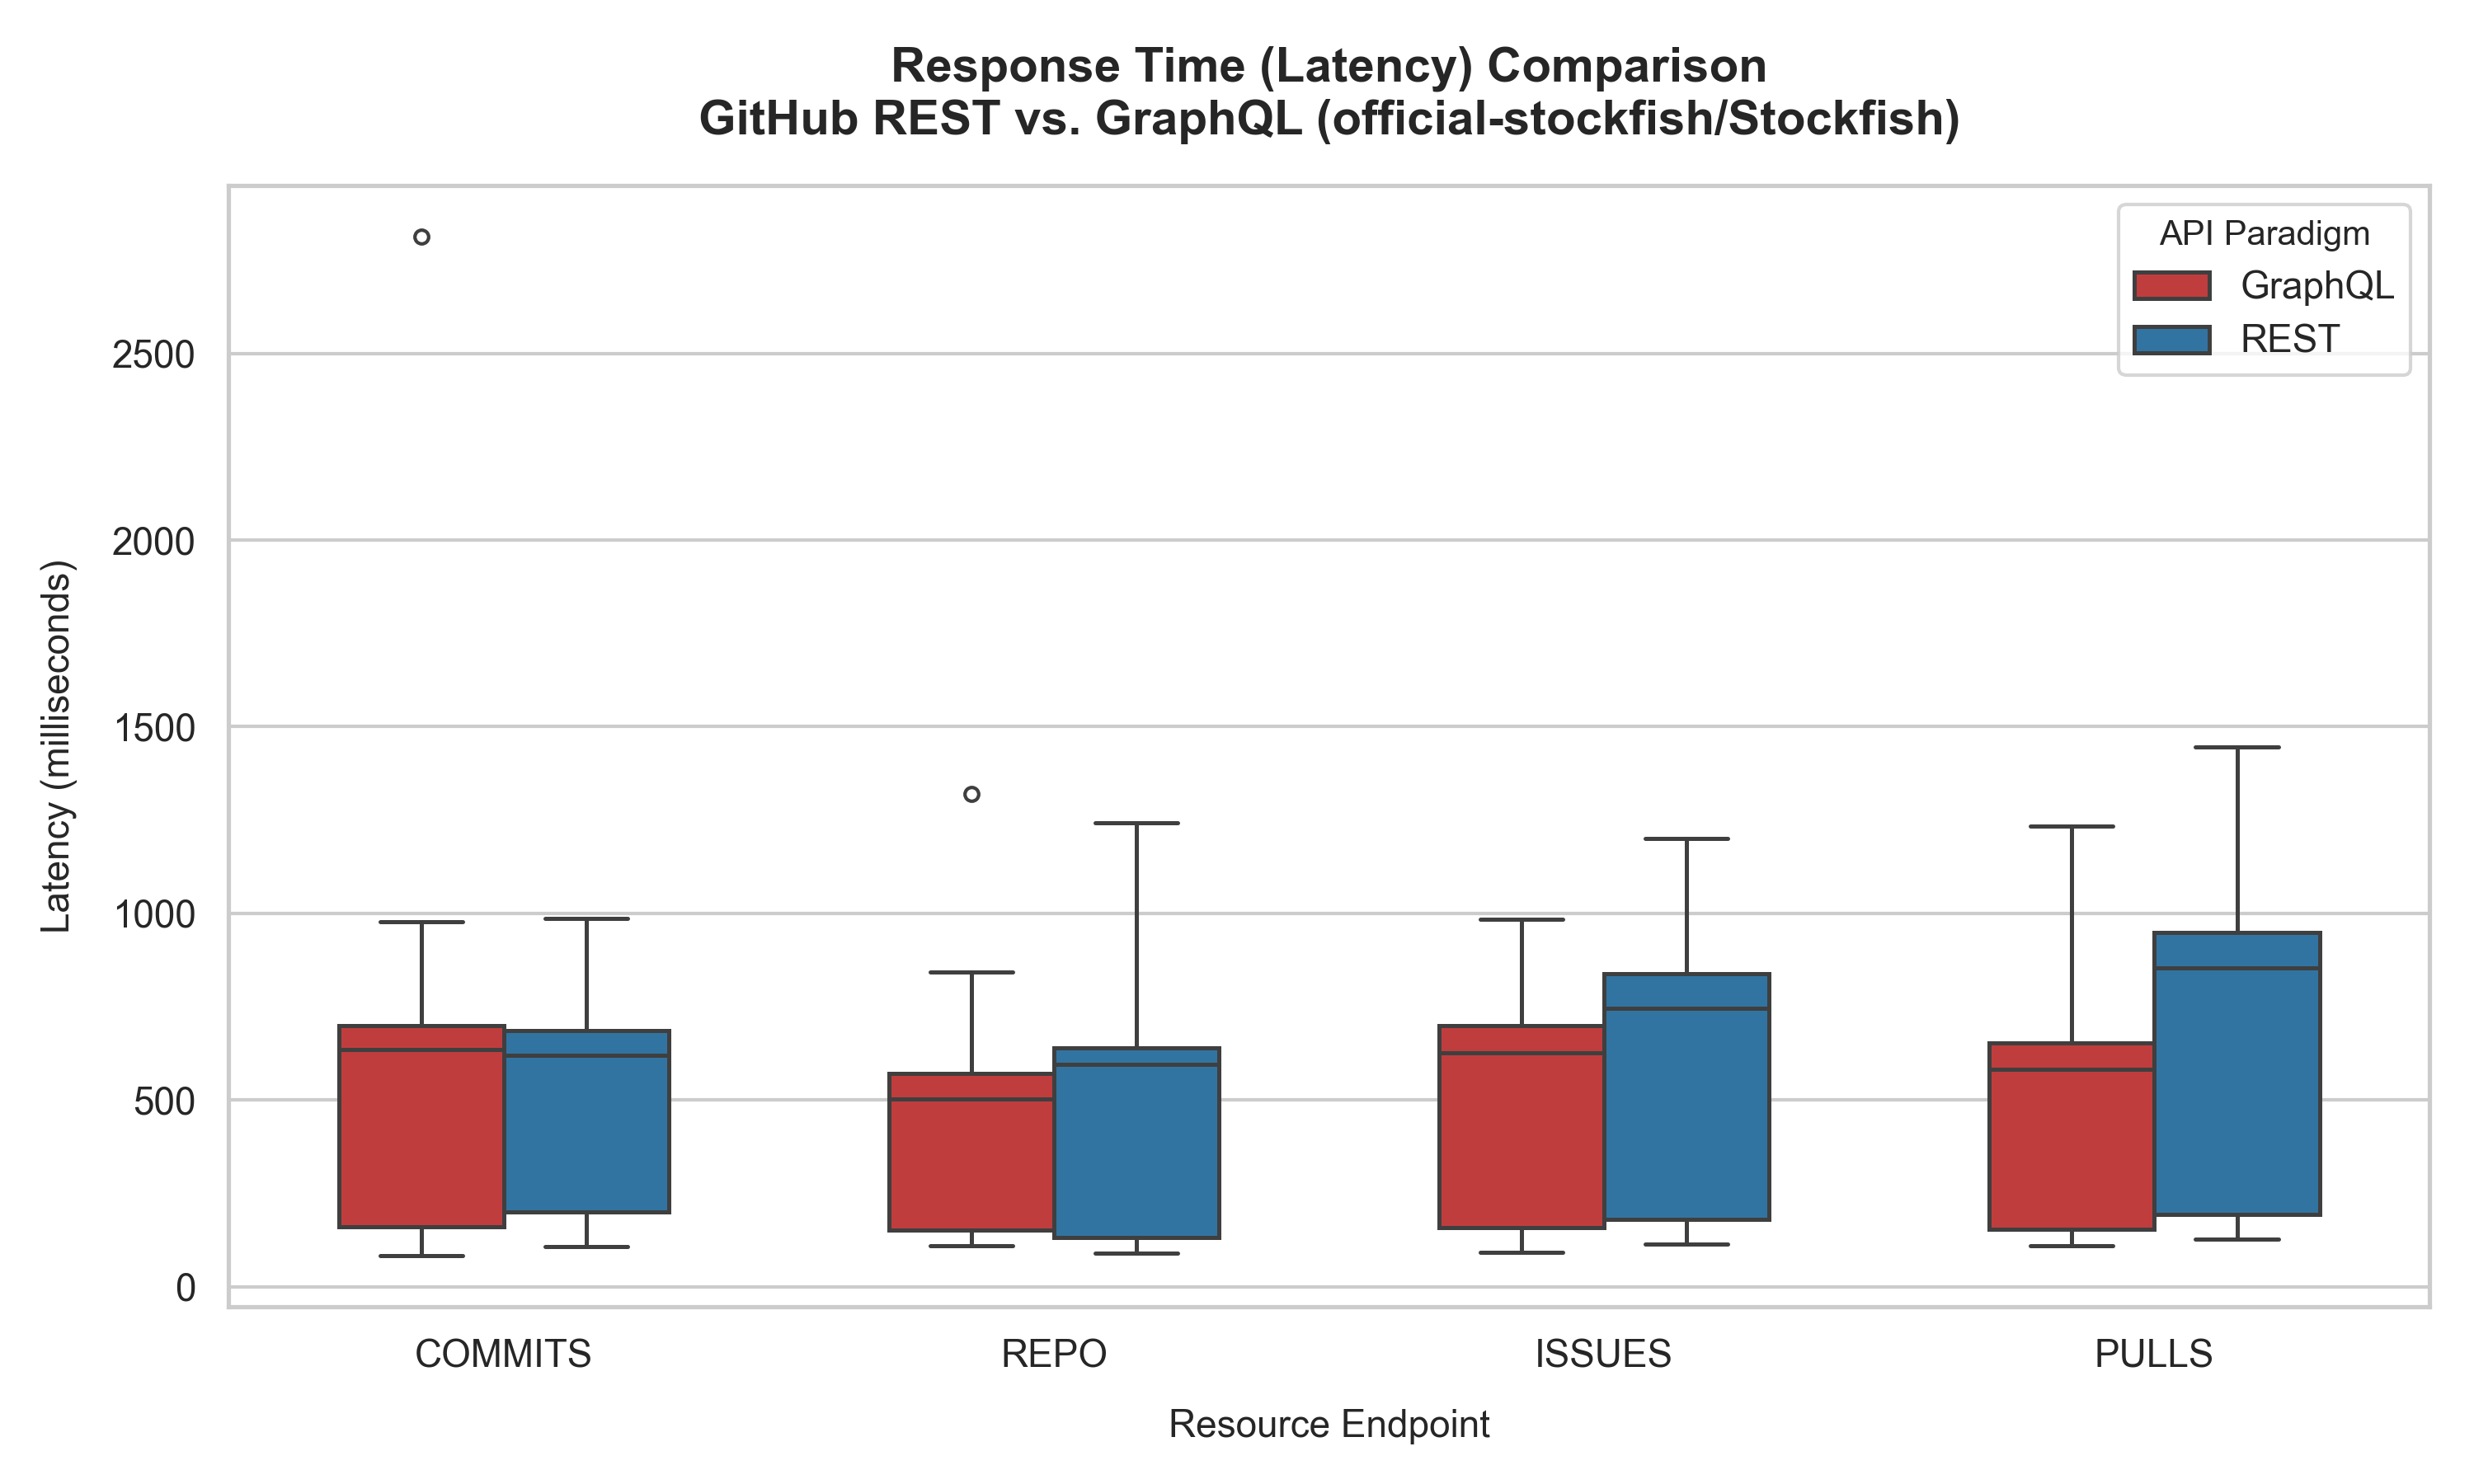
\includegraphics[width=\columnwidth]{figs/latency_comparison.png}
  \caption{Distribuição da latência (ms) por recurso e paradigma. GraphQL é
  significativamente mais rápido em \texttt{pulls} (***) e \texttt{issues}
  (**); sem diferença significativa em \texttt{repo} e \texttt{commits}.}
  \label{fig:latency}
\end{figure}

\begin{itemize}
  \item \textbf{repo} --- sem diferença significativa
    ($p=0,279$; $\delta=-0,062$, desprezível).
  \item \textbf{commits} --- sem diferença significativa
    ($p=0,117$; $\delta=-0,125$, desprezível).
  \item \textbf{issues} --- GraphQL mais rápido
    ($p=0,0066$; $\delta=-0,262$, pequeno).
  \item \textbf{pulls} --- GraphQL mais rápido
    ($p=5{,}68\times10^{-5}$; $\delta=-0,407$, médio).
\end{itemize}

% ─────────────────────────────────────────────────────────────────────────────
\subsection{RQ2 -- Tamanho do payload}
% ─────────────────────────────────────────────────────────────────────────────

A Tabela~\ref{tab:rq2} apresenta o teste para o tamanho do payload. O
resultado é \textbf{unânime e contundente}: em todos os recursos o GraphQL
retorna payloads significativamente menores, com tamanho de efeito
\textbf{máximo} ($\delta=-1{,}000$, ou seja, \emph{todas} as respostas GraphQL
são menores que \emph{todas} as REST) e $p<10^{-21}$.

\begin{table}[H]
  \centering
  \caption{RQ2 -- Mann-Whitney U (unilateral, GraphQL $<$ REST) para tamanho.}
  \label{tab:rq2}
  \small
  \begin{tabular}{lrrr}
    \toprule
    \textbf{Recurso} & \textbf{M.\ GQL} & \textbf{M.\ REST} & \textbf{Red.} \\
    \midrule
    repo    & 249\,B    & 6,9\,KB   & 96,4\,\% \\
    commits & 33,2\,KB  & 126,5\,KB & 73,8\,\% \\
    issues  & 5,0\,KB   & 115,7\,KB & 95,7\,\% \\
    pulls   & 3,8\,KB   & 529,1\,KB & 99,3\,\% \\
    \bottomrule
  \end{tabular}
  \\[2pt]
  {\scriptsize M.\ = mediana; Red.\ = redução da mediana (GraphQL vs.\ REST).
  Em todos os casos: $\delta=-1,000$ (grande) e $p<0,001$ (***).}
\end{table}

As Figuras~\ref{fig:size} e \ref{fig:sizelog} comparam o tamanho mediano em
escalas linear e logarítmica. Na escala linear, as barras do GraphQL são
quase imperceptíveis frente ao REST -- evidência visual da diferença de
\emph{ordem de grandeza}, tornada legível pela escala logarítmica.

\begin{figure}[H]
  \centering
  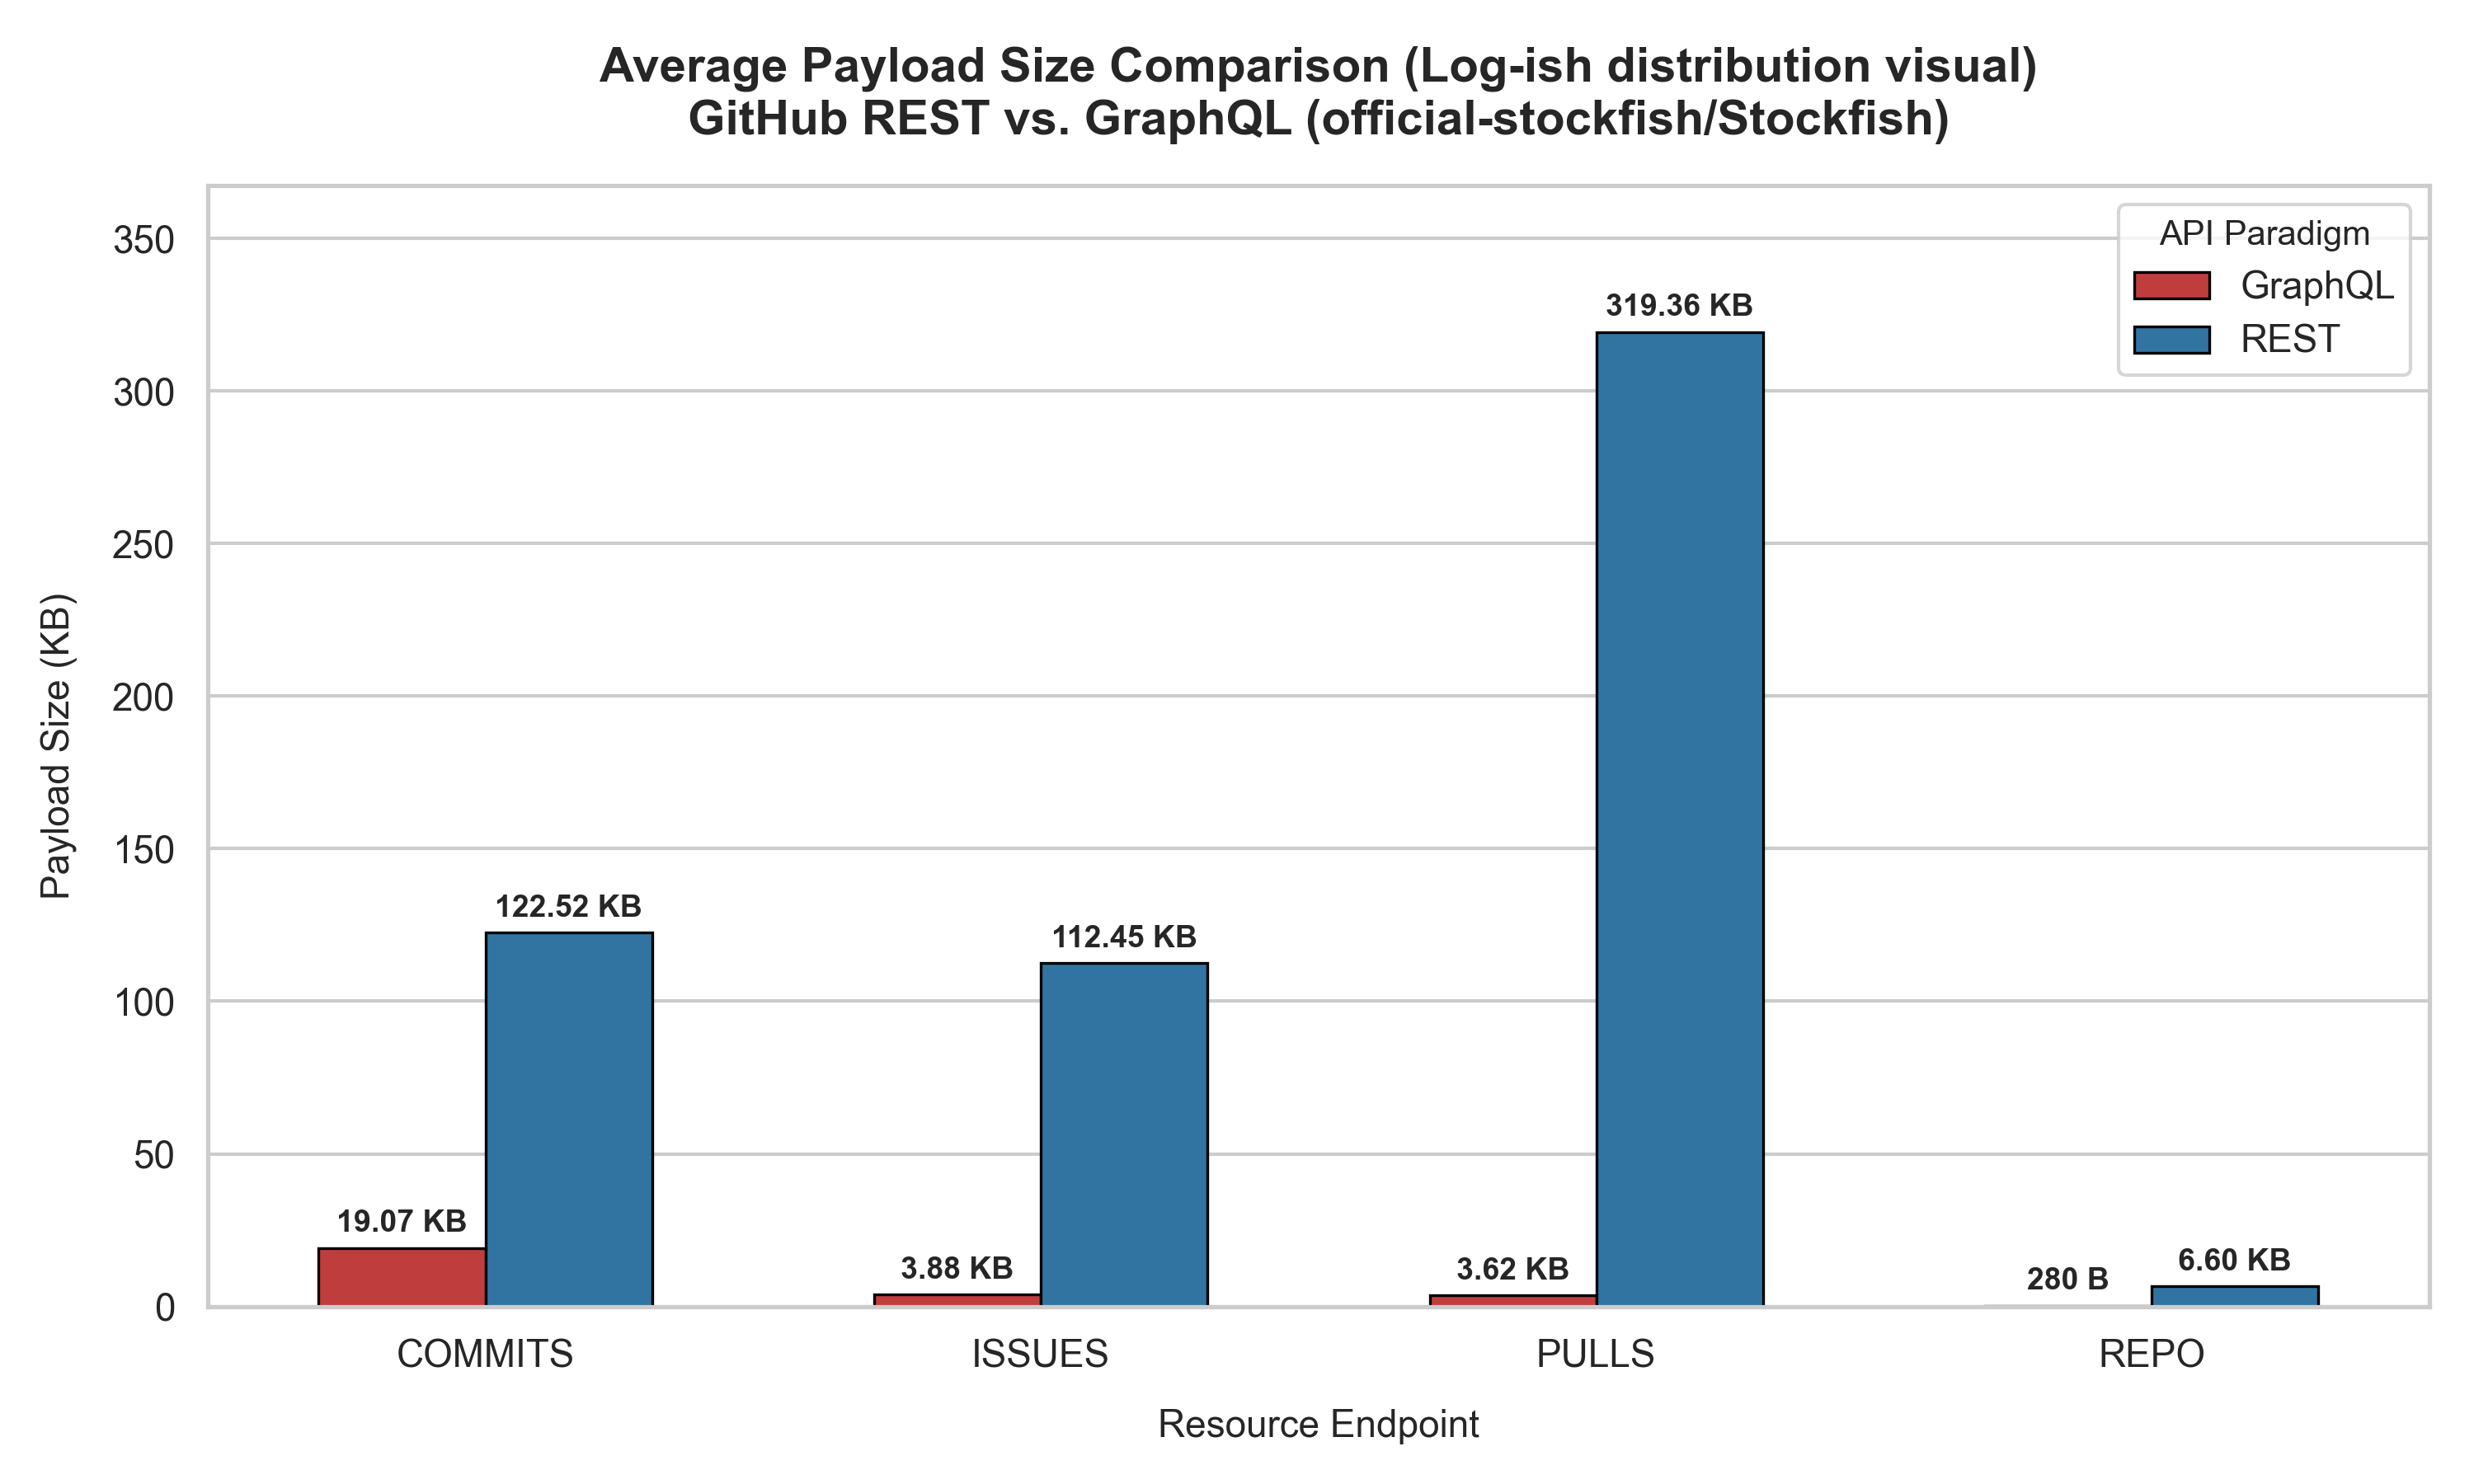
\includegraphics[width=\columnwidth]{figs/size_comparison.png}
  \caption{Tamanho mediano do payload por recurso (escala linear). A barra do
  GraphQL é praticamente nula diante do REST.}
  \label{fig:size}
\end{figure}

\begin{figure}[H]
  \centering
  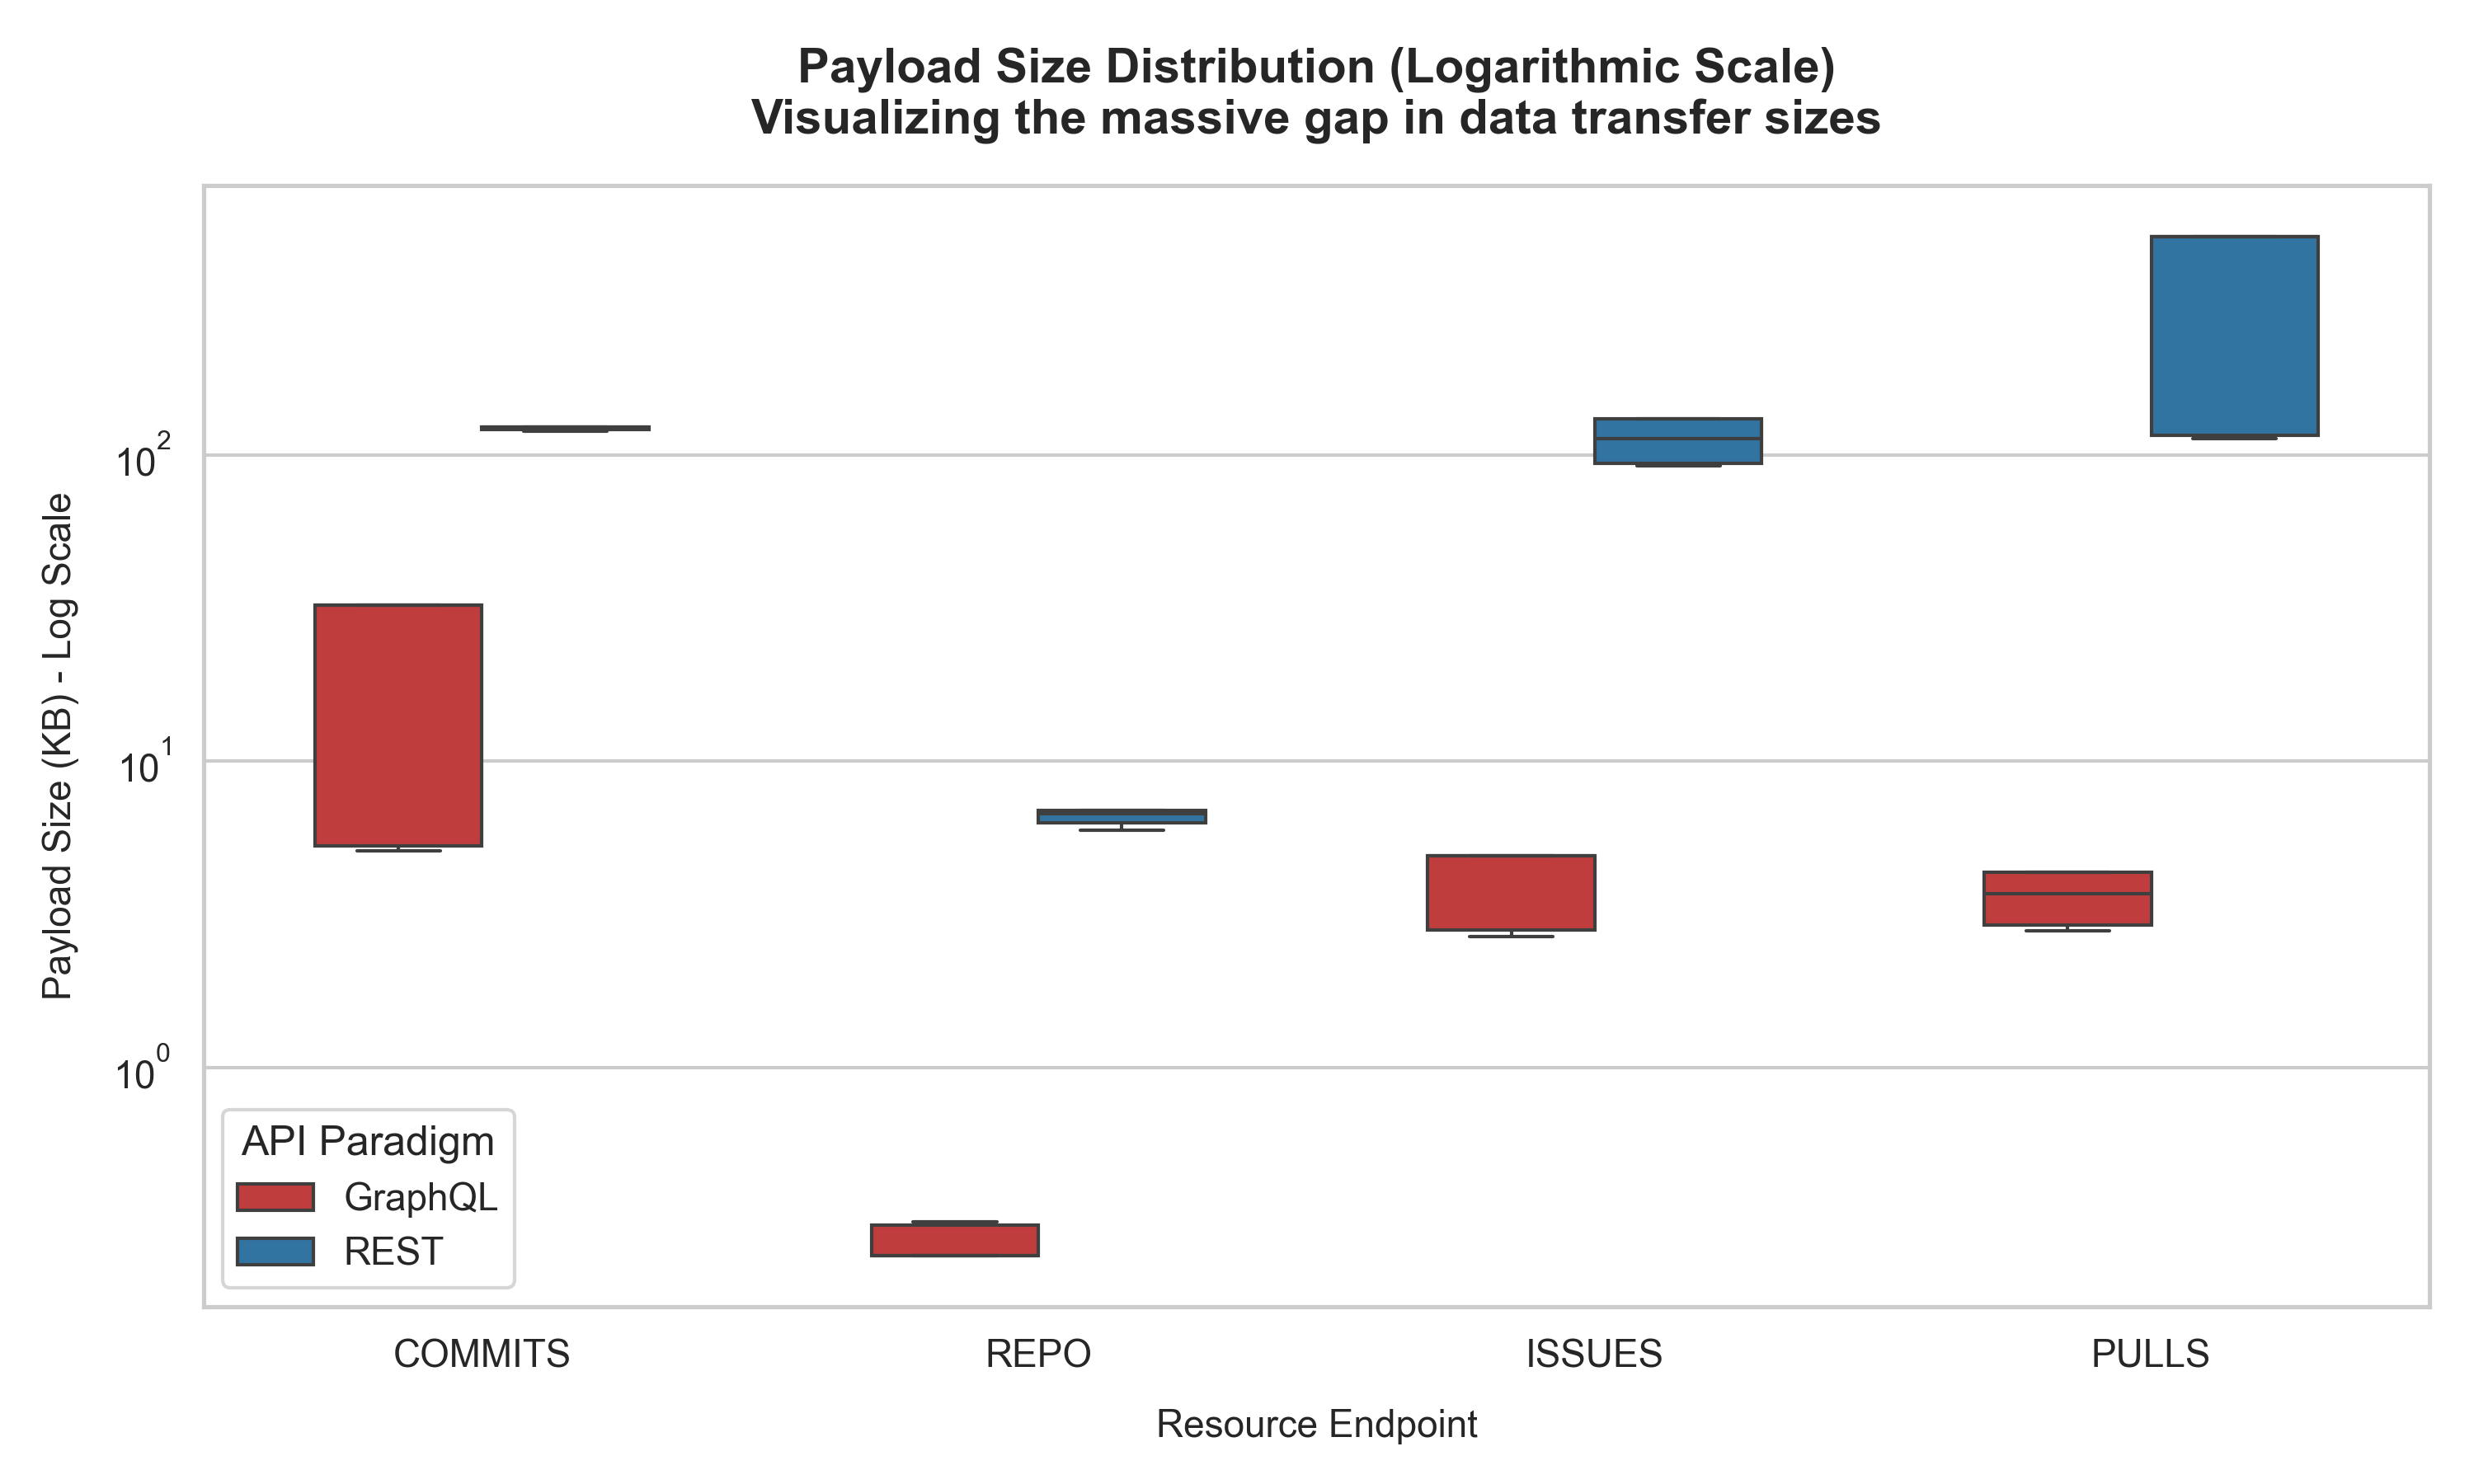
\includegraphics[width=\columnwidth]{figs/size_comparison_log.png}
  \caption{Tamanho mediano do payload por recurso (escala logarítmica),
  evidenciando a diferença de ordem de grandeza entre os paradigmas.}
  \label{fig:sizelog}
\end{figure}

\begin{itemize}
  \item \textbf{repo} --- redução de 96,4\,\% (249\,B vs.\ 6,9\,KB; ***).
  \item \textbf{commits} --- redução de 73,8\,\% (33,2\,KB vs.\ 126,5\,KB; ***).
  \item \textbf{issues} --- redução de 95,7\,\% (5,0\,KB vs.\ 115,7\,KB; ***).
  \item \textbf{pulls} --- redução de 99,3\,\% (3,8\,KB vs.\ 529,1\,KB; ***).
\end{itemize}

% ─────────────────────────────────────────────────────────────────────────────
\section{Discussão dos Resultados}
% ─────────────────────────────────────────────────────────────────────────────

\subsection{Interpretação}

\begin{itemize}
  \item \textbf{O ganho de banda é a vantagem dominante.} A redução do payload
    é consistente, de grande efeito e estatisticamente inquestionável em todos
    os recursos. A economia agregada de 95,2\,\% confirma que a prevenção de
    \textit{over-fetching} é o principal benefício prático do GraphQL.

  \item \textbf{O ganho de latência é real, porém condicional.} O GraphQL só
    foi mais rápido onde a resposta REST é volumosa (\texttt{pulls},
    \texttt{issues}), sugerindo que parte do ganho de tempo decorre do
    \emph{menor volume transferido}, não de processamento intrinsecamente mais
    rápido. Em recursos pequenos, o custo fixo de rede domina e anula a
    vantagem.

  \item \textbf{Magnitude de efeito acompanha o volume.} O Cliff's Delta da
    latência cresce em módulo de \texttt{repo} ($-0,062$) a \texttt{pulls}
    ($-0,407$), na mesma ordem em que cresce a diferença de tamanho dos
    payloads -- um indício de causalidade entre volume e tempo.
\end{itemize}

\subsection{Ameaças à Validade}

\begin{itemize}
  \item \textbf{Validade interna:} \textit{jitter} de rede e \textit{cache} de
    CDN podem inflar latências. Mitigamos com randomização total, intercalação,
    cabeçalho \texttt{no-cache} e atraso entre chamadas.
  \item \textbf{Validade de construto:} a comparação só é justa se ambas as
    APIs retornam o \emph{mesmo} conteúdo lógico; por isso as \textit{queries}
    GraphQL foram desenhadas para espelhar os campos exibidos pelo REST.
  \item \textbf{Validade externa:} os resultados refletem a infraestrutura de
    larga escala do GitHub sob internet pública e não se generalizam
    automaticamente a APIs locais ou de outras arquiteturas.
\end{itemize}

% ─────────────────────────────────────────────────────────────────────────────
\section{Conclusão e Resposta às Hipóteses}
% ─────────────────────────────────────────────────────────────────────────────

O experimento, com 487 medições válidas sobre o repositório
\texttt{official-stockfish/Stockfish}, permite responder às questões de
pesquisa:

\begin{itemize}
  \item \textbf{RQ1 (latência):} hipótese $H_{1,1}$
    \textbf{parcialmente confirmada}. Rejeitamos $H_{0,1}$ em \texttt{issues}
    e \texttt{pulls} (GraphQL mais rápido), mas não em \texttt{repo} e
    \texttt{commits}.
  \item \textbf{RQ2 (tamanho):} hipótese $H_{1,2}$
    \textbf{totalmente confirmada}. Rejeitamos $H_{0,2}$ em todos os recursos,
    com efeito máximo ($\delta=-1,000$) e economia agregada de 95,2\,\%.
\end{itemize}

A Tabela~\ref{tab:hipoteses} sintetiza o desfecho de cada hipótese.

\begin{table}[H]
  \centering
  \caption{Síntese da avaliação das hipóteses.}
  \label{tab:hipoteses}
  \small
  \begin{tabularx}{\columnwidth}{lXl}
    \toprule
    Hip. & Descrição resumida & Status \\
    \midrule
    $H_{1,1}$ & GraphQL apresenta menor latência que REST. & Parcial \\
    $H_{1,2}$ & GraphQL apresenta payload menor que REST. & Confirmada \\
    \bottomrule
  \end{tabularx}
\end{table}

\paragraph{Recomendação.} Para aplicações sensíveis a banda -- clientes
móveis, redes limitadas ou cenários de alto volume de requisições -- a adoção
do GraphQL é fortemente recomendada pelo ganho expressivo de payload. Já o
ganho de \emph{tempo} deve ser esperado sobretudo em consultas a recursos de
resposta volumosa; em recursos pequenos, a diferença de latência tende a ser
irrelevante.

\end{document}
